\documentclass[10pt,a4paper]{amsart}

\usepackage[utf8]{inputenc}
\usepackage[francais]{babel}
\usepackage[T1]{fontenc}
\usepackage{amsmath}
\usepackage{tikz}
\usetikzlibrary[patterns]
\usepackage{amsfonts}
\usepackage{amssymb}
\usepackage{graphicx}
\usepackage[left=2cm,right=2cm,top=2cm,bottom=2cm]{geometry}
\usepackage{multicol}
\usepackage{bm}

\newtheorem{exemple}{Exemple}
\newtheorem{theo}{Th\'eoreme}
\newtheorem{proposition}{Proposition}
\newtheorem{definition}{D\'efinition}
\newtheorem{lemme}{Lemme}
\newtheorem{remarque}{Remarque}

\def\gint{\displaystyle\int}

\usepackage[ruled]{algorithm}
\usepackage{algpseudocode}
\alglanguage{pseudocode}

\author{Brachet Matthieu}
\title{Analyse de dispersion généralisée}
\date\today

\begin{document}

\maketitle

%***********************************************
%
% Introduction
%
%***********************************************

\part{Introduction}

%***********************************************
%
% Discrétisation en espace
%
%***********************************************

\part{Discrétisation en espace}

\textit{
La résolution d'un problème continu par des voies numériques nécessité une discrétisation du problème initial. Différentes techniques ont été développées dans cet objectif, on pensera notamment aux éléments finis qui utilisent la formulation faible d'une EDP ou les volumes finis qui en emploient la forme intégrale.
}

\textit{
Dans cette partie, nous nous concentrerons sur les méthodes de différences finies qui utilisent directement la forme classique du problème. Nous présentons des méthodes d'approximation de $\partial_x \left[ . \right]$ dites classiques et les méthodes compacts (ou implicites). 
}

\textit{
Il sera mis en évidence l'importance d'employer une méthode d'ordre élevé. De plus, une analyse fréquentielle des schémas numériques sera proposée.
}

\textit{
Dans la suite, nous noterons $\tau_{(\Delta)} \left[ . \right]$ l'opérateur de translation ($\tau_{(\Delta)}\left[ u \right](x) = u(x + \Delta)$). On remarque alors facilement par développement de Taylor que :
}
\begin{equation}\label{taylor}
\tau_{(j\Delta)}\left[ . \right] = \sum_{p=0}^{\infty} \dfrac{(j \Delta)^p}{p!}\partial_x^p\left[ . \right]
\end{equation}

\section{Opérateurs d'approximation explicite}

Pour approcher explicitement l'opérateur $\partial_x \left[ . \right]$, on discrétise la fonction à dériver aux point $j\Delta$. On cherche l'opérateur d'approximation antisymétrique  $\tilde{\partial}_x \left[ . \right]$ sous la forme :

\begin{equation}\label{op_classique}
\tilde{\partial}_x \left[ . \right] = \sum_{i=1}^{N} a_i \dfrac{\tau_{(i\Delta)} \left[ . \right] - \tau_{(-i\Delta)} \left[ . \right]}{2i \Delta}
\end{equation}

En employant la formule \eqref{taylor} et en identifiant les coefficients, on remarque que $a=(a_1, ..., a_N)^T$ vérifie le système :

\begin{equation}\label{systeme_op_classique}
Qa=b
\end{equation}

avec $b=(1, 0, ..., 0)^T$ et 
$Q=\begin{pmatrix}
1 & 1   & 1   & \ldots & 1   \\ 
1 & 2^2 & 3^2 & \ldots & N^2 \\ 
1 & 2^4 & 3^4 & \ldots & N^4 \\ 
\vdots & \vdots & \vdots &  & \vdots \\ 
1 & 2^{2(M-1)} & 3^{2(M-1)} & \ldots & N^{2(M-1)}
\end{pmatrix} \in \mathcal{M}_{M,N}\left( \mathbb{R} \right)$

Cette identification permet, lorsque $M$ est inversible, d'obtenir une méthode d'ordre $2M$. Une condition pour avoir $M$ inversible est $M=N$. Cette méthode permet d'obtenir un schéma d'ordre $N$ totalement explicite à $2N+1$ points. 

Par exemple, pour avoir :

\begin{itemize}
\item une méthode d'ordre 2 à 3 points, on prend $a = \left( 1 \right)$,\\

\item une méthode d'ordre 4 à 5 points, on prend $a = \begin{pmatrix}
4/3 \\ -1/3
\end{pmatrix}$,\\

\item une méthode d'ordre 6 à 7 points, on prend $a = \begin{pmatrix}
3/2 \\ -3/5 \\ 1/10
\end{pmatrix}$.

\end{itemize} 

Avec ces trois exemples, on obtient les approximations suivantes :

\begin{itemize}
\item à l'ordre 2 :
\begin{equation}\label{explicite ordre 2}
\dfrac{u(x+\Delta)-u(x-\Delta)}{2\Delta} = \partial_x \left[ u \right](x) + \mathcal{O}\left( \Delta^2 \right)
\end{equation}\\

\item à l'ordre 4 :
\begin{equation}\label{explicite ordre 4}
\dfrac{4}{3}\dfrac{u(x+\Delta)-u(x-\Delta)}{2\Delta} - \dfrac{1}{3}\dfrac{u(x+2\Delta)-u(x-2\Delta)}{4\Delta} = \partial_x \left[ u \right](x) + \mathcal{O}\left( \Delta^4 \right)
\end{equation}\\

\item à l'ordre 6 :
\begin{equation}\label{explicite ordre 6}
\dfrac{3}{2}\dfrac{u(x+\Delta)-u(x-\Delta)}{2\Delta} - \dfrac{3}{5}\dfrac{u(x+2\Delta)-u(x-2\Delta)}{4\Delta} + \dfrac{1}{10}\dfrac{u(x+3\Delta)-u(x-3\Delta)}{6\Delta} = \partial_x \left[ u \right](x) + \mathcal{O}\left( \Delta^6 \right)
\end{equation}

\end{itemize} 

Il est évident qu'une discrétisation d'ordre plus élevé sera nettement plus précise. Le choix de la discrétisation utilisé est crucial dans une méthode numérique.

\section{Opérateur d'approximation compact}

Les schémas implicite, aussi appelés \textit{Hermitiens} ou \textit{Compacts}, sont introduit par Sanjiva K. Lele \cite{Lele} en 1991. Nous présentons ici l'idée générale mais une étude plus détaillée sera présentée ultérieurement.

On considère toujours que l'on souhaite approcher $\partial_x \left[ . \right]$ à l'aide d'un nouvel opérateur discret $\tilde{\partial}_x \left[ . \right]$. Ce dernier est définit de manière implicite par une relation de la forme :


\begin{equation}\label{op_implicite}
\alpha_0 \tilde{\partial}_x \left[ . \right] + \sum_{j=1}^{M} \alpha_j \left(\tau_{(j\Delta)} \left[ \tilde{\partial}_x \left[ . \right] \right] + \tau_{(-j\Delta)} \left[ \tilde{\partial}_x \left[ . \right] \right] \right) = \sum_{i=1}^{N} a_i \dfrac{\tau_{(i\Delta)} \left[ . \right] - \tau_{(-i\Delta)} \left[ . \right]}{2i \Delta}
\end{equation}

Les inconnues étant ici $\left( \alpha_j \right)_{0 \leq j \leq M}$ et $\left( a_i \right)_{1 \leq i \leq N}$.

L'inconvénient des méthodes implicites réside en la nécéssité de résoudre un système linéaire pour calculer l'approximation. La résolution de se système linéaire peut se faire à l'aide d'un solveur rapide tel que l'algorithme de Thomas lorsque la partie implicite est tridiagonale ($M=1$). Dans un cadre général, cette résolution de système peut demander un fort coût en calcul.

En fait, on note que les $\left(a_i\right)_{1 \leq i \leq N}$ peuvent être donnés par une première approximation de $\partial_x \left[ . \right]$. Ils sont alors issus du système \eqref{systeme_op_classique} donné dans la partie précédente. Dans ce cadre, les $\left(a_i\right)_{1 \leq i \leq N}$ sont déterminés, il reste donc à résoudre :

\begin{equation}
\alpha_0 \delta_{0,p} + \sum_{i=1}^{L} \alpha_i \dfrac{i^{p+1} + (-i)^{p+1}}{(p+1)!} = \sum_{i=1}^{N} a_i \dfrac{i^{p+1} - (-i)^{p+1}}{2(p+2)!}
\end{equation}

qui se ramène à la résolution d'un système linéaire lorsque les $(a_i)_{1 \leq i  \leq N}$ sont donnés par \eqref{systeme_op_classique} ($\delta_{0,p}$ est le symbole de Kronecker).
On peut trouver les schémas compacts suivants :

\begin{itemize}
\item Schéma d'ordre 4 :
\begin{itemize}
\item $a = \left( 1 \right)$\\
\item $\alpha = \begin{pmatrix}
2/3 \\ 1/6
\end{pmatrix}$
\end{itemize}

\item Schéma d'ordre 6 :
\begin{itemize}
\item $a = \begin{pmatrix}
4/3 \\ -1/3
\end{pmatrix}$\\
\item $\alpha = \begin{pmatrix}
4/5 \\ 2/15 \\ -1/30
\end{pmatrix}$
\end{itemize}
\end{itemize}

De nombreux schémas explicites existent. Sanjiva K. Lele les présente sous une autre forme dans \cite{Lele}, il donne aussi une famille de schémas compacts à 7 points explicites et 3 points implicites (l'emploi de l'algorithme de Thomas est alors possible), ces derniers sont alors donnés par les relations :

\begin{equation}
\left\{
\begin{array}{rcl}
a_1 & = & 2 \alpha_1 + 4 \alpha_0 \\
3 a_2 & = & 4 \alpha_1 - \alpha_0 \\
\end{array}
\right.
\end{equation}

et tous les autres coefficients nuls. De plus, il existe des schémas explicites optimisés au sens fréquentiel, ces derniers sont présentés dans \cite{Tam Webb} et \cite{Redonnet}. 

\section{Analyse fréquentielle}

On sait qu'un signal $u$ se décompose suivant les harmoniques. En consèquence, on considère une quantité harmonique de pulsation $\omega$ et de vitesse de phase $c$ :

$$\widehat{s}(x,t) = |\widehat{s}| e^{i \omega \left( \frac{x}{c} - t \right)}$$

En posant le nombre d'onde $k=\omega / c$, on peut directement réécrire :

$$\widehat{s}(x,t) = |\widehat{s}| e^{i \left( k x - \omega t \right)}$$

L'erreur de troncature est donnée par :

$$\varepsilon_t = \partial_x \left[ \widehat{s} \right] - \tilde{\partial}_x \left[ \widehat{s} \right]$$

Il est facil de voir que $\partial_x \left[ \widehat{s} \right] = ik \widehat{s}$. De plus, on remarque que $\tau_{(j \Delta)} \left[ \widehat{s} \right] = e^{i k j \Delta} \widehat{s}$.

Ainsi, on peut écrire :

\begin{equation}
\tilde{\partial}_x \left[ \widehat{s} \right] = \dfrac{i}{\Delta} \dfrac{\sum_{j=1}^{N} a_j sin\left( j k \Delta \right) }{  \alpha_0 + 2 \sum_{j=1}^{M} \alpha_j cos \left( j k \Delta \right) } \left[ \widehat{s} \right]
\end{equation}

Ainsi, si on pose $\theta = k \Delta$, on doit avoir :

\begin{equation}\label{nombre d'onde approché}
\theta \approx \tilde{\theta} \left( \theta \right) = \dfrac{\sum_{j=1}^{N} \dfrac{a_j}{j} sin\left( j \theta \right) }{  \alpha_0 + 2 \sum_{j=1}^{M} \alpha_j cos \left( j \theta \right) }.
\end{equation}

Observons dans le cadre des différents exemples précédents la qualité de cette approximation.
Par des dévellopements de Taylors simples, on trouve les résultats suivants pour les exemples précédents :



\textbf{Schémas explicites}
   
\begin{itemize}
\item à l'ordre 2 :
$$\tilde{\theta}(\theta) = \theta - \dfrac{\theta^3}{6} + \mathcal{O} \left( \theta^5 \right)$$

\item à l'ordre 4 :
$$\tilde{\theta}(\theta) = \theta - \dfrac{\theta^5}{30} + \mathcal{O} \left( \theta^7 \right)$$

\item à l'ordre 6 :
$$\tilde{\theta}(\theta) = \theta - \dfrac{\theta^7}{140} + \mathcal{O} \left( \theta^9 \right)$$

\end{itemize}
   
\textbf{Schémas implicites}
   
\begin{itemize}
\item à l'ordre 4 :
$$\tilde{\theta}(\theta) = \theta - \dfrac{\theta^5}{180} + \mathcal{O} \left( \theta^7 \right)$$

\item à l'ordre 6 :
$$\tilde{\theta}(\theta) = \theta - \dfrac{\theta^7}{630} + \mathcal{O} \left( \theta^9 \right)$$
\end{itemize}

De plus, on remarque triviallement que la fonction $\tilde{\theta}$ est impaire et $2 \pi-$périodique. On peut s'intérésser à la représentation du coefficient modifié $\theta$ en fonction de $\theta$.

Pour les différents exemples donnés ci dessus, les résultats graphiques sont donnés en figure \ref{LOM}


\begin{figure}[h!]
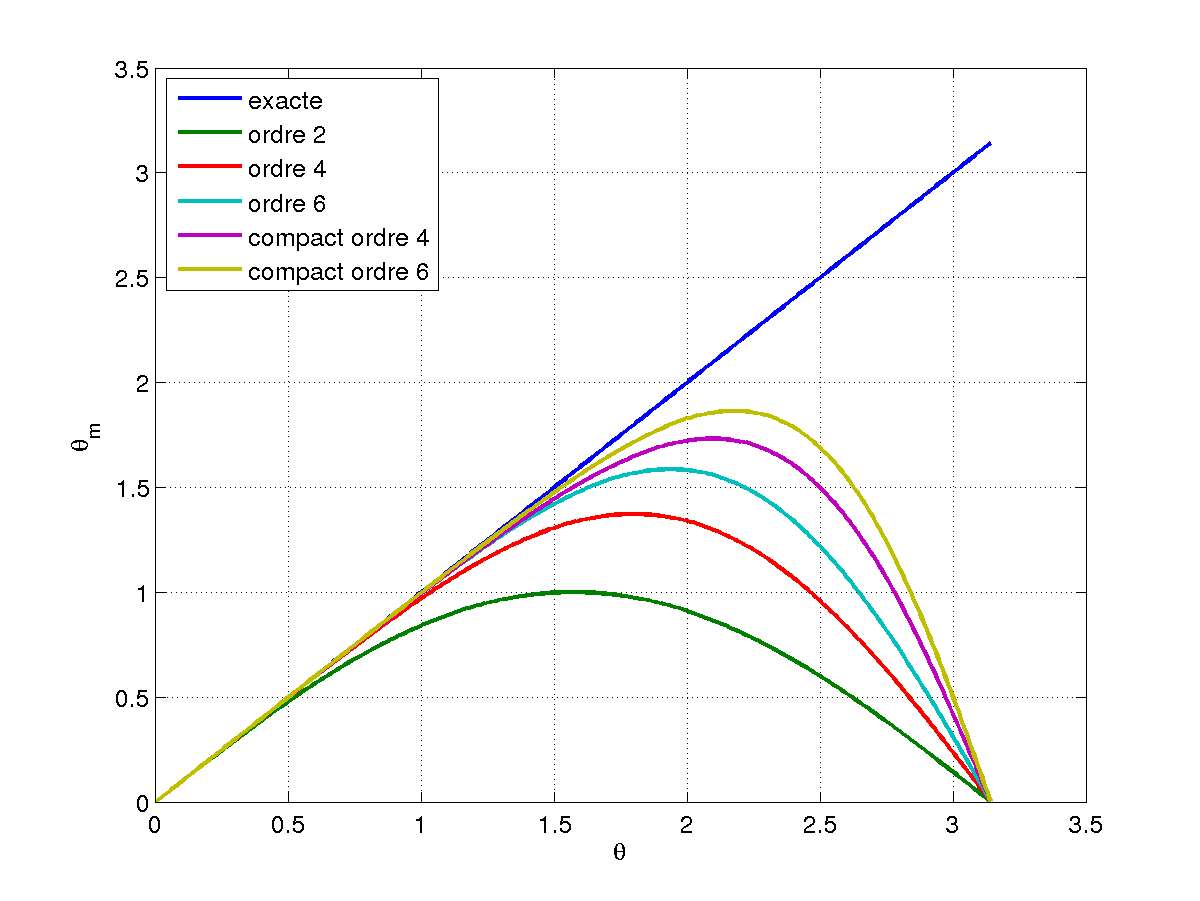
\includegraphics[scale=0.4]{onde_modifiee.png}
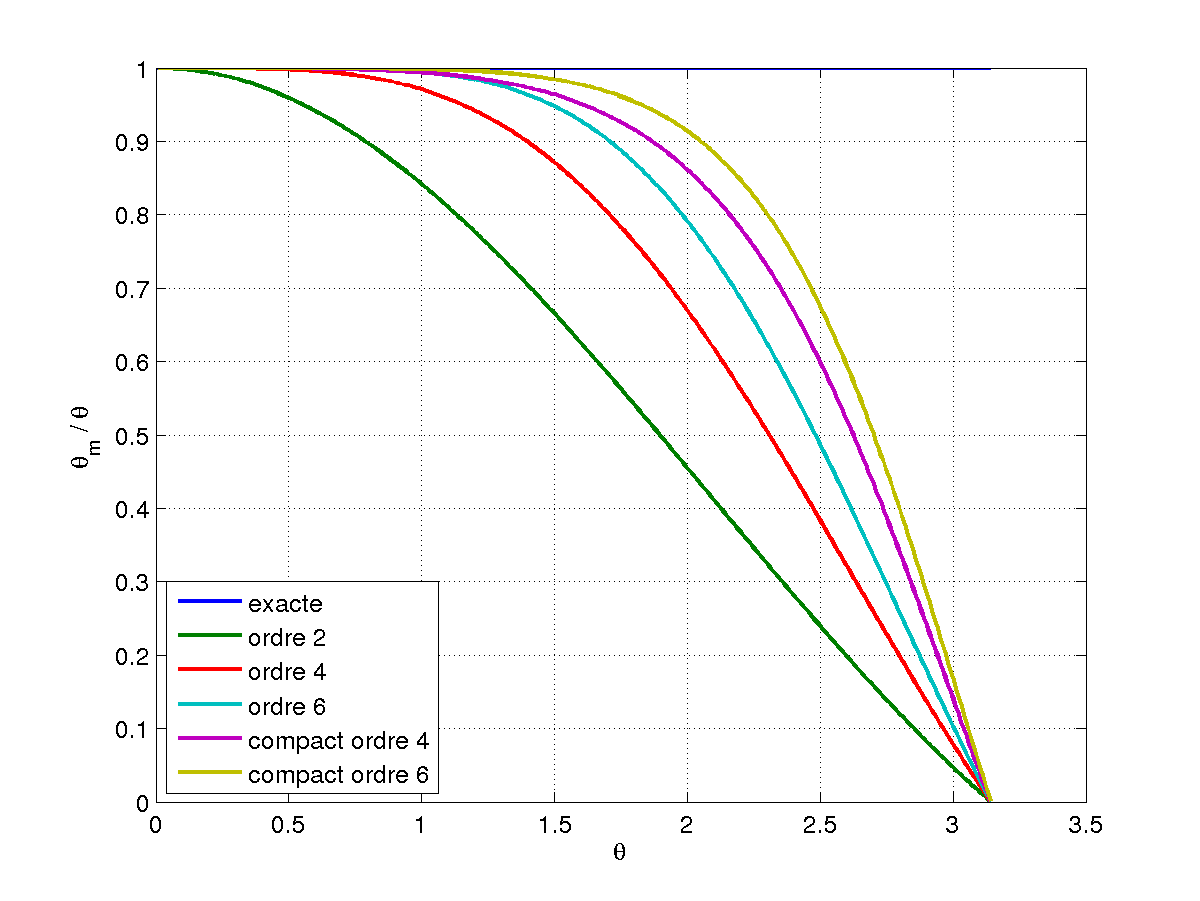
\includegraphics[scale=0.4]{coef_onde_modifiee.png}
\caption{$\theta$ modifiée par différents schémas en espace}
\label{LOM}
\end{figure}

On observe facilement que plus un schéma est précis plus il "colle" à la courbe $\theta$. Mais un autre points doit être évoqué. On observe que les schémas compacts donnent une approximation supérieure à celle donnée par les schémas explicites. A ordre de précision identique, il est plus précis d'utiliser un schéma compact plutot qu'un schéma explicite classique : les hautes fréquences sont mieux représentées.


%***********************************************
%
% Discrétisation en temps
%
%***********************************************

\part{Discrétisation en temps}

Une fois la discrétisation spatiale effectuée, une EDP semi-discrétisée peut etre vue comme une EDO. Par exemple, pour l'équation de transport :

$$\dfrac{\partial u}{\partial t} + c \dfrac{\partial u}{\partial x}$$

en notant $D$ l'opérateur discret d'approximation de $\partial / \partial x$, on obtient :

$$\dfrac{\partial u}{\partial t} = -c D \cdot u$$

Dans le cadre des EDO, comme dans celui des EDO, il est donc important de pour voir discrétiser la partie temporelle. Les méthodes de Runge-Kutta sont parmis les méthodes de discrétisations temporelles les plus performantes connues. Elles permettent en effet de calculer à une précision importante la solution approchée. Des méthodes permettant un faible stockage ont été dévellopées, on citera en particulier \cite{Kennedy Carpenter Lewis}. Les méthodes classiques de Runge-Kutta sont en particulier expliquées dans le livre de Jean-Pierre Demailly \cite{Demailly}.

\section{Méthode de type Runge-Kutta}

L'objectif des méthodes de Runge-Kutta est de calculer la solution approchée de l'équation aux dérivées ordinaires (EDO) :

\begin{equation}\label{EDO}
\left\{
\begin{array}{rcl}
u' & = & F(t,u)\\
u(t=0) & = & u_0
\end{array}
\right.
\end{equation}

Pour $t \in \left[ 0, T \right]$. On discrétise $\left[ 0, T \right]$ en intervalles $\left[ t^n, t^{n+1} \right]$ de longueur $\Delta t$ et on cherche à approcher $u(t^n)$ pour tout $n$. Notons $u^n$ cette approximation.

En intégrant \eqref{EDO}, on remarque que :

$$
\begin{array}{rcl}
u(t^{n+1}) & = & u(t^n) + \gint_{t^n}^{t^{n+1}} F(t, u(t))dt\\
           & = & u(t^n) + \gint_{0}^{1} F(t^n + \alpha \Delta t, u(t^n + \alpha \Delta t)) d \alpha
\end{array}
$$

On emploie alors une formule de quadrature pour approcher l'intégrale :

\begin{equation}\label{RK_quadratureglobale}
\gint_{0}^{1} F(t^n + \alpha \Delta t, u(t^n + \alpha \Delta t)) d \alpha \simeq \sum_{1 \leq j < q} b_j F(t^{n,j}, u(t^{n,j}))
\end{equation}

où les $t^{n,j}$ sont des temps intermédiaires inclus dans $\left[ t^n, t^{n+1} \right]$. La difficulté réside alors dans l'impossibilité de déterminer $u(t^{n,j})$ exactement.

Pour déterminer ces valeurs intermédiaires au temps $t^{n,j} = t^n + c_j \Delta t$, on procéde de la même manière avec la formule de quadrature :

\begin{equation}\label{RK_quadratureglobale}
u^{n,i} = u^n + \Delta t \sum_{1 \leq j < i} a_{i,j} F(t_j, u^{n,j}))
\end{equation}

L'algorithme de calcul est le suivant :

 \begin{center}
\begin{minipage}[H]{12cm}
  \begin{algorithm}[H]
    \caption{: Explicit Runge-Kutta Method's}\label{RK}
    \begin{algorithmic}[1]
        \State $u^0 = u^{(0)}$ given
            \For{$n=0,1, \ldots$}
              \For {$i=1, \ldots , q$}
             \State  $t^{n,i} = t^n + c_i \Delta t$
             \State  $u^{n,i} = u^n + \Delta t \sum_{1 \leq j < i} a_{i,j} K_j$
             \State  $K_i = F(t^{n,i}, u^{n,i})$ 
             \EndFor
              \State $u^{n+1} = u^n + \Delta t \sum_{1 \leq i \leq q} b_i K_i$           
            \EndFor
    \end{algorithmic}
    \end{algorithm}
\end{minipage}
\end{center}

Il est fréquent de nommer les coefficients $a_{i,j}$, $b_j$ et $c_i$ les coefficients de Butcher et de les représenter sous la forme d'un tableau comme ci-dessous :

\begin{table}[h!]
\begin{center}
$\begin{array}{c|ccccc}
c_1 & 0 & 0 & \cdots & 0 & 0 \\
c_2 & a_{2,1} & 0 & \cdots & 0 & 0 \\
\vdots & \vdots & \vdots & \ddots & \vdots & \vdots \\
\vdots & \vdots & \vdots &  & 0 & 0 \\
c_q & a_{q,1} & a_{q,2} & \cdots & a_{q, q-1} & 0 \\
\hline
    & b_1  & b_2 & \cdots & b_{q-1} & b_q 
\end{array}$
\caption{Tableau de Butcher}
\label{rk_butcher}
\end{center}
\end{table}

On note que nous n'avons présenté ici que les méthodes de Runge-Kutta explicites à pas constant. D'autres méthodes plus ou moins stables et précises existent.

Les méthodes de Runge-Kutta explicites les plus classiques sont (respectivement à l'ordre 1, 2 et 4) :

\begin{itemize}
\item \textbf{Méthode d'Euler Explicite :}

\begin{center}
$\begin{array}{c|c}
0 & 0 \\
\hline
  & 1 \\
\end{array}$
\end{center}

\item \textbf{RK2 : }
\begin{center}
$\begin{array}{c|cc}
0 & 0 & 0\\
\alpha & \alpha & 0 \\
\hline
  & 1-\frac{1}{2 \alpha} & \frac{1}{2 \alpha} \\
\end{array}$
\hspace{1cm} où $\alpha \in \left] 0, 1 \right]$.
\end{center}


\item \textbf{RK4 : }
\begin{center}
$\begin{array}{c|cccc}
0 & 0 & 0 & 0 & 0\\
1/2 & 1/2 & 0 & 0 & 0 \\
1/2 & 0 & 1/2 & 0 & 0 \\
1 & 0 & 0 & 1 & 0 \\
\hline
  & 1/6 & 2/6 & 2/6 & 1/6 \\
\end{array}$
\end{center}

\end{itemize}

\section{Conditions sur l'ordre des méthodes de Runge-Kutta}

Commençons par définir $\Phi$ par :

$$u^{n+1} = u^n  + \Delta t \Phi(t^n,u^n,\Delta t)$$

où $(u^n)_n$ est une suite définie par une méthode de Runge-Kutta.

Une méthode est consistante si et seulement si :

$$\forall \left( t, u \right) \in \left[ 0, T \right] \times \mathbb{R}, \hspace{0.8cm} \Phi(t,u,0) = F(t, u)$$

Dans le cas des méthodes de Runge-Kutta, cela revient à dire que :

$$\sum_{i=1}^q b_i = 1$$

En fait, plus généralement, on dira qu'une méthode est consistante à l'ordre $p$ si pour toute solution exacte $u$ de \eqref{EDO} où $F \in \mathcal{C}^p$, il existe $C > 0$ telle que l'erreur de consistance véérifie :

$$|e_n| \leq C \Delta t^{p+1}$$

où l'erreur de consistance est donnée par :

$$e_n = u(t^{n+1}) - u(t^n) - \Delta t \Phi(t^n,u(t^n),\Delta t)$$

Si $\Phi \in \mathcal{C}^p$, par dévellopement de Taylor, on a facilement :

$$\Phi(t^n,u(t^n),\Delta t) = \sum_{k=0}^{p} \dfrac{\Delta t^k}{k!} \dfrac{\partial^k \Phi}{\partial \Delta} (t^n, u(t^n), 0) + o \left( \Delta t^p  \right)$$

De la même manière, on a :

$$u(t^{n+1}) - u(t^n) = \sum_{k=0}^{p} \dfrac{1}{(k+1)!} F^{[k]}(t^n, u(t^n))) + o \left( \Delta t^{p+1}  \right)$$

Où $F^{[k]}$ est la $k-$ième dérivée de $z(t)=F(t, u(t))$ et où $u$ vérifie \eqref{EDO}. De là, on déduit qu'une méthode est d'ordre supérieur ou égal à $p$ si et seulement si la relation suivante est vérifiée pour tout $k \leq p-1$ :

\begin{equation}
\dfrac{\partial^k \Phi}{\partial \Delta^k} (t, y, 0) = \dfrac{1}{k+1}F^{[k]}(t,y)
\end{equation}

De là, on peut déduire un résultat général sur les méthodes de Runge-Kutta explicites.

La méthode de Runge-Kutta donnée par le tableau de Butcher \ref{rk_butcher} est  :

\begin{itemize}
\item \textbf{d'ordre au moins 1} si :
$$\sum_{i} b_i = 1$$
\item \textbf{d'ordre au moins 2} si la condition précédente est vérifiée ainsi que :
$$\sum_{j} b_j c_j = \dfrac{1}{2}$$
\item \textbf{d'ordre au moins 3} si les conditions précédentes sont vérifiées ainsi que :
\begin{center}
$\sum_j b_j c_j^2 = \dfrac{1}{3}$ et $\sum_{i,j} b_i a_{i,j} c_j = \dfrac{1}{6}$
\end{center}
\item \textbf{d'ordre au moins 4} si les conditions précédentes sont vérifiées ainsi que :
\begin{center}
$\sum_j b_j c_j^3 = \dfrac{1}{4}$, $\sum_{i,j} b_i a_{i,j} c_j^2 = \dfrac{1}{12}$, $\sum_{i,j} b_i c_i a_{i,j} c_j = \dfrac{1}{8}$ et $\sum_{i,j,k} b_i a_{i,j} a_{j,k} c_k = \dfrac{1}{12}$
\end{center}
\end{itemize}

Grâce à ces conditions, on peut vérifier facilement qu'Euler Explicite est d'ordre 1, RK2 est d'ordre 2 et RK4 est d'ordre 4.

\section{Analyse de stabilité sur un exemple}

La stabilité absolue d'une méthode linéaire à 1 pas est donnée par la condition :

\begin{equation}
|u^{n+1}| \leq |u^n|
\end{equation}

où $u^n$ est donné par une méthode de Runge-Kutta.

Traitons les exemples précédents dans le cas de l'équation :

\begin{equation}\label{EDO_simple}
\left\{
\begin{array}{rcl}
u' & = & \beta u \\
u(t=0) & = & u_0
\end{array}
\right.
\end{equation}

La solution de cette équation est trivialement donnée par $u(t)=u_0 e^{\beta t}$. Dans la suite, nous posons $\lambda = \beta \Delta t \in \mathbb{C} $.

Une méthode de Runge-Kutta à $q$ étapes est donnée par (pour l'équation \eqref{EDO_simple}) :

\begin{equation}\label{RK_edo_simple}
K_i = \beta \left( u_n + \Delta t \sum_{j=1}^{q} a_{i,j}K_j \right) \text{, } u_{n+1} = u_n + \Delta t \sum_{i=1}^q b_i K_i
\end{equation}

Si on pose $\bm{K} = (K_1, ..., K_q)^T$ et $\bm{1} = (1, ..., 1)^T$ alors \eqref{RK_edo_simple} s'écrit :

\begin{equation}\label{RK_matriciel}
\bm{K} = \beta \left( u_n \bm{1} + \Delta t A \bm{K} \right) \text{, } u_{n+1} = u_n + \Delta t b^T \bm{K}
\end{equation}

d'où on tire facilement $\bm{K} = (I + \lambda A)^{-1}) \bm{1} u_n$ et :

$$u_{n+1} = \left[ 1 + \lambda \bm{b}^T (I + \lambda A)^{-1} \bm{1} \right] u_n = R(\lambda) u_n $$

On apelle zone de stabilité absolue la région où :

$$\mathcal{A} = \left\{ \lambda \in \mathbb{C} \text{ t.q. } \dfrac{|u_{n+1}|}{|u_n|} = |R(\lambda)| < 1 \right\}$$

La méthode est stable si et seulement si $|R(\lambda)| < 1$. Or comme la méthode est ici explicite, $A$ est triangulaire inférieure stricte et l'égalité suivante est vérifiée :

$$R(\lambda) = \dfrac{det(I - \lambda A + \lambda \bm{1} \bm{b}^T)}{det(I - \lambda A)} = det(I - \lambda A + \lambda \bm{1} \bm{b}^T)$$

Ainsi, $R(\lambda)$ est un polynome en $\lambda$. Une méthode de Runge-Kutta ne peut donc pas être stable pour toutes les valeurs de $\lambda$.

Voici quelques exemples de régions de stabilité :



\begin{itemize}
\item \textbf{Euler explicite : }

$$|1 + \lambda| \leq 1$$

\item \textbf{RK2 :}

$$|1+\lambda(2 - \dfrac{1}{2 \alpha} + \alpha \lambda)| \leq 1$$

\item \textbf{RK4 :}

Si on pose $K_1 = \lambda$, $K_2 = \lambda (1 + \dfrac{1}{2}K_1)$, $K_3 = \lambda (1 + \dfrac{1}{2}K_2)$ et $K_4 = \lambda (1 + K_3)$ alors la région de stabilité est donnée par :

$$|1 + \dfrac{1}{6} \left( K_1 + 2 K_2 + 2 K_3 + K_4 \right)| \leq 1$$
\end{itemize}

On peut avoir les représentations graphiques suivantes :


\begin{figure}[!h]
\begin{center}
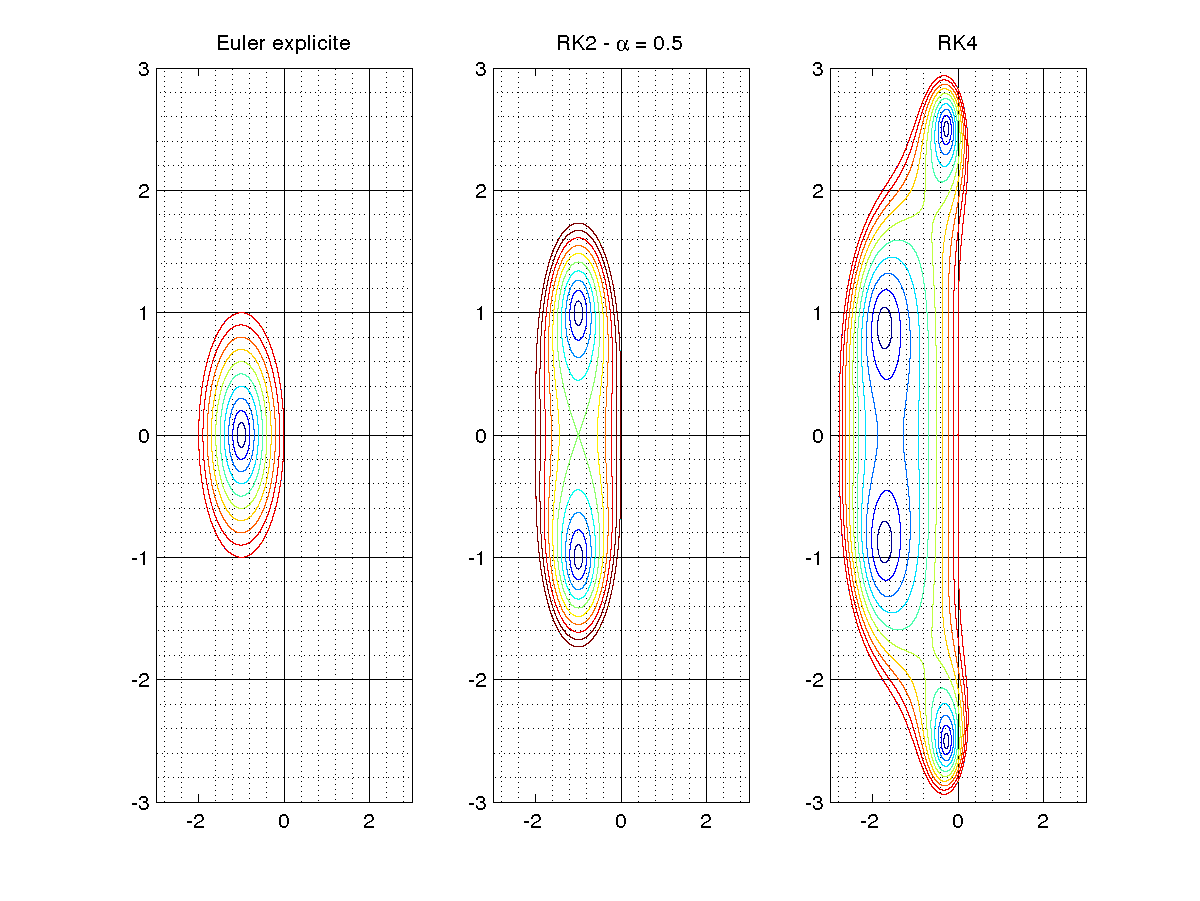
\includegraphics[scale=0.6]{rk_stab.png}
\caption{Régions de stabilité pour pour Euler Explicite (gauche), RK2($\alpha = 0.5$) (centre) et RK4 (gauche)}
\end{center}
\end{figure}

%***********************************************
%
% Diffusion et Dispersion numérique
%
%***********************************************

\part{Diffusion et Dispersion numérique}

Pour introduire les notions de diffusion et dispersion numérique, on utilise l'équation de convection (transport) ci-dessous :

\begin{equation}\label{eq transport}
\dfrac{\partial u}{\partial t} + c \dfrac{\partial u}{\partial x} = 0
\end{equation}

munie d'une condition initiale qui ne nous intéresse pas ici.
On discrétise cette solution sur un maillage $\left( i \Delta x, n \Delta t \right)$. On a alors $u_i^n$ une approximation de $u(i \Delta x, n \Delta t )$.

Si la méthode est d'ordre $p$ en temps et $q$ en espace, l'erreur de consistance est sous la forme suivante :

$$\left[ \text{schéma numérique} \right] - \left[ \dfrac{\partial u}{\partial t} + c \dfrac{\partial u}{\partial x} \right] = T \Delta t^p \dfrac{\partial^{p+1} u}{\partial t^{p+1}} + c E \Delta x^q \dfrac{\partial^{q+1} u}{\partial t^{q+1}} + \ldots$$

Si $\Delta t$ et $\Delta x$ sont fixés, l'équation résolue n'est pas vraiment \eqref{eq transport} mais une équation équivalente de la forme :

\begin{equation}\label{equation modifiee}
\dfrac{\partial u}{\partial t} + c \dfrac{\partial u}{\partial x} + Q \Delta^\alpha \dfrac{\partial^{\alpha + 1} u}{\partial x^{\alpha + 1}}= 0 
\end{equation}

où $\alpha = min(p,q)$ et $\Delta = \Delta t$ si $p<q$ et inversement. $Q$ est une quantité dépendant de $T$, $E$ et $c$. Cette équation est directement issue de l'erreur de consistance, en prenant en compte que $u$ est solution de \eqref{eq transport}.
\newline


\section{Diffusion numérique : }

Lorsque $\alpha$ est impair, on obtient une éqution modifiée de type convection-diffusion. Plus le coefficient de viscosité $Q \Delta^{\alpha}$ est grand, plus le schéma est \textit{diffusif}. Bien qu'une loi de conservation puisse admettre des discontinuités, la présence du terme :
$$Q \Delta^\alpha \dfrac{\partial^{\alpha + 1} u}{\partial^{\alpha + 1} x}$$
 entraine une certaine régularité dans la solution numérique. Les discontinuités seront "étalées" plus étalées dans l'espace lorsque $Q \Delta^{\alpha}$ est grand.
\newline


\section{Dissipation numérique : }

A l'inverse, lorsque $\alpha$ est pair, il apparait des coefficients de dispersion numérique. Comme l'équation est linéaire \eqref{equation modifiee}, on peut s'intéressé à chaque mode de Fourier et chercher la solution sous la forme d'une harmonique :

$$u(x,t)= e^{i(kx - \omega t)}$$

On obtient la relation de dispersion suivante :

\begin{equation}
\omega = ck + Q \left( i \Delta \right)^{\alpha} k^{\alpha +1}
\end{equation}

On note que $\omega \in \mathbb{R}$ car $\alpha$ est pair. On remarque que chaque mode de Fourier se déplace à une vitesse $c_p = \omega / k = c + Q \left( i \Delta k \right)^{\alpha}$ qui dépend de $k$. Donc chaque mode de Fourier se déplace à une vitesse \textit{a priori} différente, ils sont dispersés au cours du temps.

Lorsque $Q \Delta$ est proche de $0$ cette dispersion est amoindrie car $\omega / k$ est proche de $c$.

Dans la pratique lorsque $c_p < c$, les différentes longueurs d'onde vont moins vite que les discontinuités. On observe l'apparition d'oscillations en aval des chocs.

\section{Approximation en espace temps de l'équation de Transport}


%***********************************************
%
% Filtrage des hautes fréquences
%
%***********************************************

\part{Filtrage des hautes fréquences}

\section{Filtres explicites en espace}

\section{Analyse fréquentielle}



%***********************************************
%
% Hyperviscosité
%
%***********************************************

\part{Hyperviscosité}

\section{Idée générale}

\section{Application}








\newpage

\begin{thebibliography}{9}
        

\bibitem{Redonnet}
         Stéphane Redonnet
         \emph{:  Simulation de la propagation acoustique en présence d'écoulements quelconques et de structures soludes par résolution numérique des équations d'Euler}.
         Thèse,
         2364,
         2001.
         
\bibitem{Kennedy Carpenter Lewis}
         Christopher A. Kennedy, Mark H. Carpenter, R. Michael Lewis
         \emph{:  Low-storage, explicit Runge-Kutta schemes for the compressible Navier-Stokes equation}.
         Applied Numerical Mathematics,
         2000.
         
\bibitem{Demailly}
         Jean-Pierre Demailly
         \emph{:  Analyse numérique et équations différentielles}.
         édition EDP,
         Collection Grenoble Sciences
         2006.
         
\bibitem{Cook Cabot 1}
         Andrew W. Cook, William H. Cabot
         \emph{:  A hight-wavenumber viscosity for hight-resolution numerical methods}.
         Journal of computational physics,
         2004.
         
\bibitem{Cook Cabot 2}
         Andrew W. Cook, William H. Cabot
         \emph{:  Hyperviscosity for shock-turbulence interactions}.
         Journal of computational physics,
         2005.
         
\bibitem{Tam Webb}
         Christopher K. W. Tam, Jay C. Webb
         \emph{:  Dispersion-Relation-Preserving Finite Difference Schemes for computational acoustics}.
         Journal of computational physics,
         1992.
         
\bibitem{Lele}
         Sanjiva K. Lele
         \emph{:  Compact Finite Difference Schemes with Spectral-like Resolution}.
         Center for turbulence Research, NASA-Ames Research Center
         Journal of computational physics,
         1991.
         
\bibitem{Goncalves}
         Eric Goncalvès
         \emph{:  Résolution numérique des équations d'Euler monodimensionnelles}.
         Cours de l'Institut Polytechnique de Grenoble,
         ENSE3,
         2008.

		
\end{thebibliography}

\end{document}